\section{The Clang Static Analyzer}

\emph{Clang} is an open-source compiler, which is based on the \emph{LLVM} 
project \cite{lattner:clang}. This is a quickly improving project, 
supported by various companies including e.g. Google, Apple, Samsung, Ericsson, 
etc.
Since Clang is built outstandingly modular, it is not simply a compiler but a 
complete framework for creating developer tools on C/C++/Objective-C 
languages. Its API is well documented and the software is well tested due to 
the wide user base.


The Clang Static Analyzer (CSA) -- as it is indicated by its name -- build 
around the Clang compiler. It is one of the most quickly developing open source 
static analysis tool. In this section the principles and the relevant 
implementation details of the CSA will be presented.

\subsection{Symbolic execution}
The CSA uses the symbolic execution static analysis algorithm which means it 
simulates the possible execution paths and tries make conclusions. It basically 
interprets the source code but instead of using the actual semantics, it 
defines an abstract one and models the state according to the defined one.

Unknown values is represented by symbols/symbolic values. The CSA makes 
constraints on these symbolic values during the analysis of the different 
paths. Among others, these constraints came from the condition on which a path 
may bifurcate. There is a constraint solver module in the analyzer which 
handles these and tries to deduce the conflicts (exclude the non-feasible 
paths). This is important since a bug found on a non-feasible path is 
considered as a false positive. The analysis stops if all of the execution 
paths are simulated and checked or it reaches a predefined limit.

The memory is represented by a hierarchic memory region system 
\cite{clang:memmodel}, the correspondence between symbolic values and memory 
regions is tracked. The state of a given program point contains this relation 
of bindings as well.

\begin{figure}[h]
	\centering
	\frame{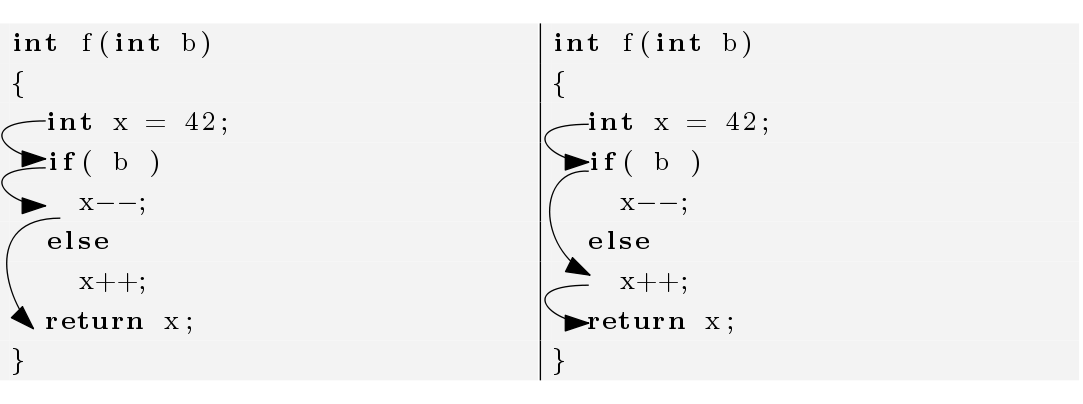
\includegraphics[width=1\textwidth]{img/utvonalak}}
	\caption{The different execution paths of a simple function}
	\label{fig:exec_path}
\end{figure}

The analysis of the different execution paths can be done in any order, 
however, the evaluation of an expression (on a given path) must happen 
according to the language standard.  
During the simulation of the expressions the analyzer models the state of the 
program, means that one expression/instruction will create a transition between 
two states. A symbolic state can be viewed as a set of concrete program states, 
moreover, a simulated path is basically an analysis of these symbolic states in 
a well defined order. 

In order to be able to perform this process efficiently, the analyzer creates 
an internal model of the execution paths, called ExplodedGraph 
\cite{explodedgraph}. The nodes of the ExplodedGraph (called ExplodedNodes) are 
pairs, containing a symbolic program state and a program point. The program 
point determines the code location where the symbolic execution is in the 
source text. The directed edge between ExplodedNodes determines the sequencing.

Whenever the CSA encounters a branch in the symbolic execution, it creates new 
branches in the ExplodedGraph (see Fig \ref{fig:exploded_graph}). The paths
from the root to the leaves represents the analyzed paths. This means, that the 
number of leaves in the ExplodedGraph (and so the size of the graph) is 
exponential with respect to the branches in the execution. That results us a 
complex, precise but resource consuming method.

The ExplodedGraph is a simple directed acyclic graph. Whenever the analysis 
reachesan ExplodedNode which was already visited before, then the simulation 
will be stopped since the CSA would do the same (deterministic) reasoning what 
was already done. Note, that in case of concrete program states this would lead 
to an infinite loop, on the symbolic level this does not stand, since a
symbolic program state represents a set of real program states.

\begin{figure}[h]
	\centering
	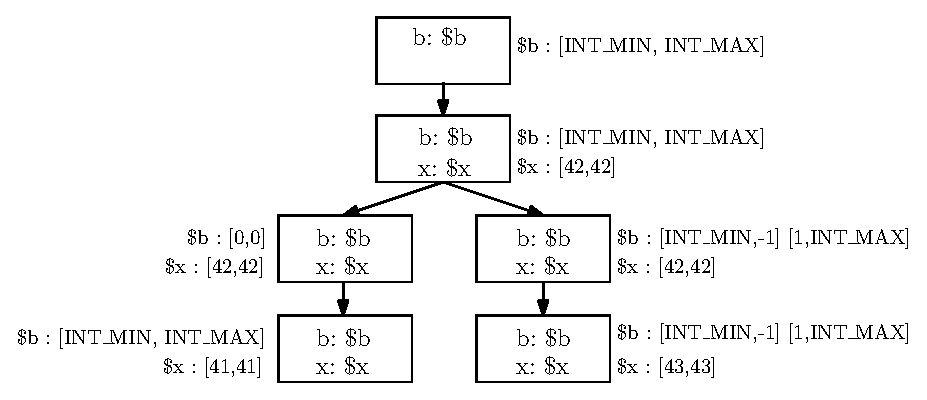
\includegraphics[width=1\textwidth]{img/explodedgraph.eps}
	\caption{The corresponding ExplodedGraph to the function presented on Fig 
		\ref{fig:exec_path}. The constraints made on the symbolic values are 
		shown next to the ExplodedNodes it belongs.}
	\label{fig:exploded_graph}
\end{figure}

In practice, the CSA constructs ExplodedNodes which does not represent any 
concrete transition between nodes but just help the simulation e.g. at some 
points the analyzer cleans up the stored but not necessary symbols and so it 
introduces a new node in order to smoothly fit this procedure into the flow of 
the analysis.

\begin{figure}[h]
	\centering
	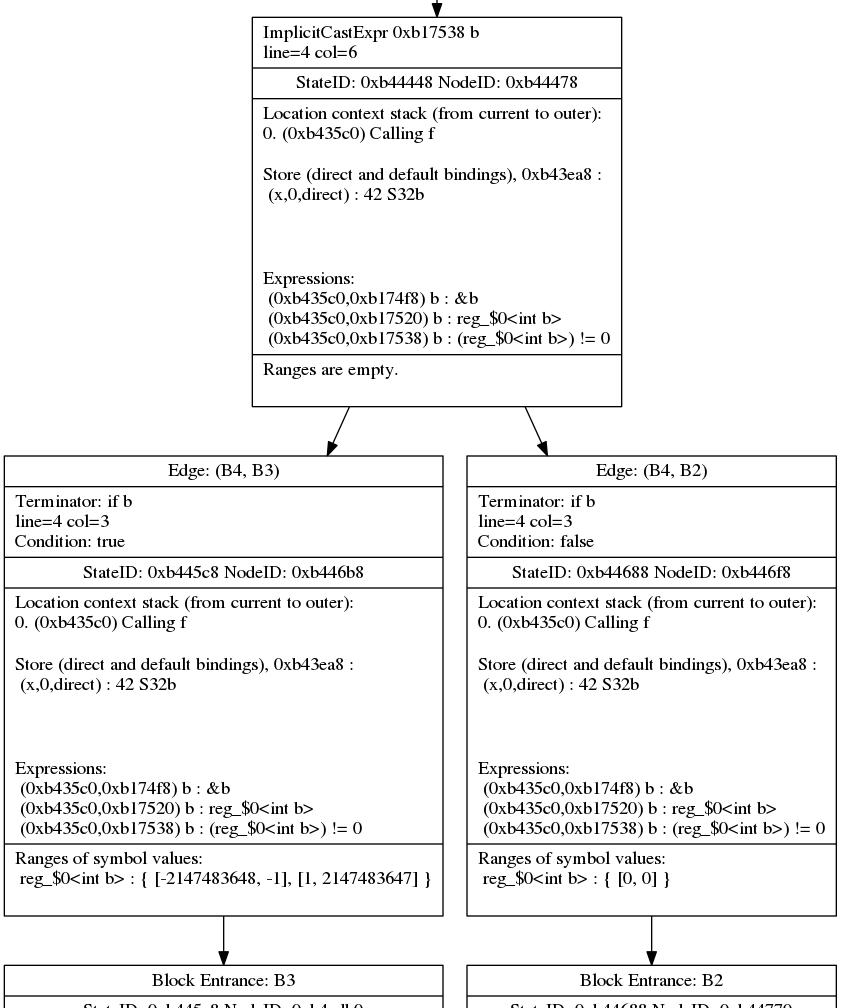
\includegraphics[width=0.7\textwidth]{img/eg}
	\caption{A small part of the actual ExplodedGraph built by the Clang 
	Static Analyzer for the function shown on Fig \ref{fig:exec_path}.}
	\label{fig:exploded_graph2}
\end{figure}

According to the properties of the model, it can be declared, that the symbolic 
execution is a path sensitive algorithm, i.e. reaching any program state the 
CSA knows the whole path leading to the simulated point. Thereby the displaying 
of the bugs shows not only the location of the bug but the corresponding 
execution path as well. This productively helps the programmer to understand 
the problem more easily, even spending less time on fixing the bug.

\begin{figure}[h]
	\centering
	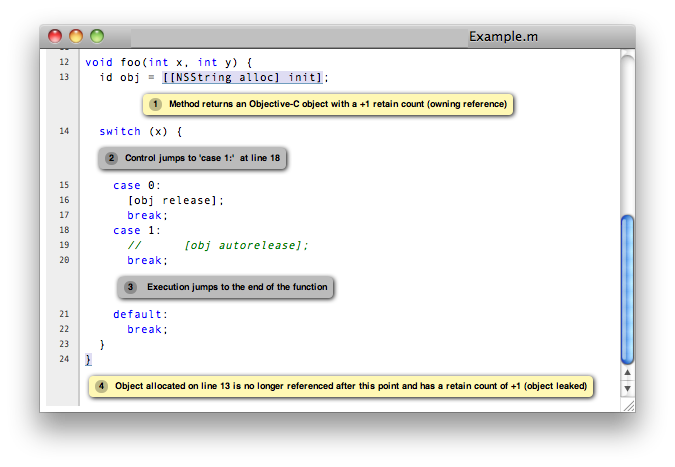
\includegraphics[width=1\textwidth]{img/view}
	\caption{A bug found by the Clang Static Analyzer can be represented in 
	HTML format to make it more clear and easier to understand.}
	\label{fig:hibak_megjelenitese}
\end{figure}

\subsection{Implementation details}
\subsubsection{The process of the analysis}
The CSA works on a translation unit, analyzing its content function by 
function. So the the internal model is constructed for an analysis of a 
function and its states are represented in the ExplodedGraph.

Whenever -- during the simulation of a given path -- the CSA encounters a 
branch in the execution, it splits the states creating more children for the 
actually simulated ExplodedNode, and so constructs new paths to analyze. 
Moreover, the condition which caused the branching is stored and the assumption 
whether it is true or false as well. This can potentially results in 
restriction on the symbolic values, and so we collect information which help us 
on the upcoming decisions. 

It is possible that the simulation encounters a call of an other function.
At this point the called function will be evaluated/analyzed on the spot of the 
call, knowing the calling context. This allows us to make a more precise 
analysis of the called function, since we potentially have information on the 
possible values of its arguments. The analysis of a function while knowing the 
calling context is called an \textit{inline} analysis. The other possibility -- 
when we have absolutely no information or precondition on the values of a 
function and it is analyzed so -- is called an \textit{top level} analysis.

In order to decrease the rate of false positive reports and make the analysis 
more time efficient, the CSA will not reanalyze a function as top level if it 
was already analyzed as an inline function. The analyzer tries to inline as 
much function as possible. This is reached by creating the function call graph 
of the translation unit and the analysis order of the functions is determined 
by a post-traversal-walk TODO on this call graph.

As it was mentioned earlier, branches in the execution lead to an exponential number of \texttt{ExplodedNode}s.
This combinatorial explosion is handled in the Static Analyzer by restricting or even stopping
the analysis when given conditions are fulfilled. Terminating the analysis 
process may cause loss of potential true positive results, but it is 
indispensable for maintaining a reasonable resource consumption regarding the 
memory and CPU usage. 

These conditions are modeled by the concept of budget.
The budget is a collection of limitations on the shape of the \texttt{ExplodedGraph}.
These limitations include:
\begin{enumerate}  
	\item The maximum number of traversed nodes in the \texttt{ExplodedGraph}. 
	If 	this number is reached then the analysis of the simulated function stops.
	\item The size of the simulated call stack. When a function call is 
	reached then the analysis continues in its body as if it was inlined to the 
	place of call (interprocedural). There are several heuristics that may control 
	the	behavior of inlining process. For example the too large functions are 
	not	inlined at all, and the really short functions are not counted in the 
	size of	call stack.
	\item The number of times a function is inlined. The idea behind this
	constraint is that the more a function is analyzed, the less likely it 
	is that a 	bug will appear in it. If this number is reached then that 
	function will not be inlined again in this \texttt{ExplodedGraph}.
	\item The number of times a basic block is processed during the 
	analysis. This	constraint limits the number of loop iterations. When this 
	threshold is reached the currently analyzed execution path is aborted. 
	(Note: only the simulation of that given path is stopped not the whole 
	analysis.)
\end{enumerate}

The budget expression can be used in two ways. Sometimes it means the
collection of the limitations above, sometimes it refers to one of these
limitations. This will always be distinguishable from the context.

\subsubsection{The building process of the model}
The syntactic and semantic information of variables, functions and types
are essential to perform the above described simulation. These informations 
required for the compilation process as well. The compilers store them in a 
data structure specially designed for this task, called abstract syntax tree 
(AST). In practice it usually contains concrete (platform specific) 
informations, and semantic properties as well, moreover, in some cases, circles 
can occur. Mainly we call it AST only because of historical reasons. 
However, the listed properties shows that having a structure like this is 
essential for the symbolic execution. That is the main motivation for building 
a static analysis tool around a compiler. An important note, that these 
structure must be well tested on a compiler since it is used for code 
generation. The CSA uses the AST build by the Clang compiler.

From the AST we are able to build an internal model, called \texttt{Control 
Flow 
Graph} (CFG). The \texttt{CFG} represents a source-level, intra-procedural 
control flow of a statement. This statement can potentially be an entire 
function body, or just a single expression. The \texttt{CFG} consists of 
\texttt{CFGBlocks} which are simply containers of statements. The 
\texttt{CFGBlocks}s essentially represent the basic blocks of the code but can 
contain some extra custom information. 
Although basic blocks and \texttt{CFGBlocks} are technically different, in the 
rest of the article the term basic blocks will be used for \texttt{CFGBlocks} 
as well for the sake of easier understanding and better illustration.

Thus based on the CFG of the functions an \texttt{ExplodedGraph} can be built.

The internal model of the execution paths is created and traversed 
simultaneously 
by an optimized depth first search. The main reason for the depth first search 
is that it allows us to memory efficiently simulate the paths, since we must 
keep the currently analyzed path in memory (in order to be able to report it as 
well). Moreover, a depth first search requires less context change than a 
breath first search which help the analysis to more efficiently cache the 
investigated symbolic values and memory regions for a given path.

\begin{figure}[h]
	\centering
	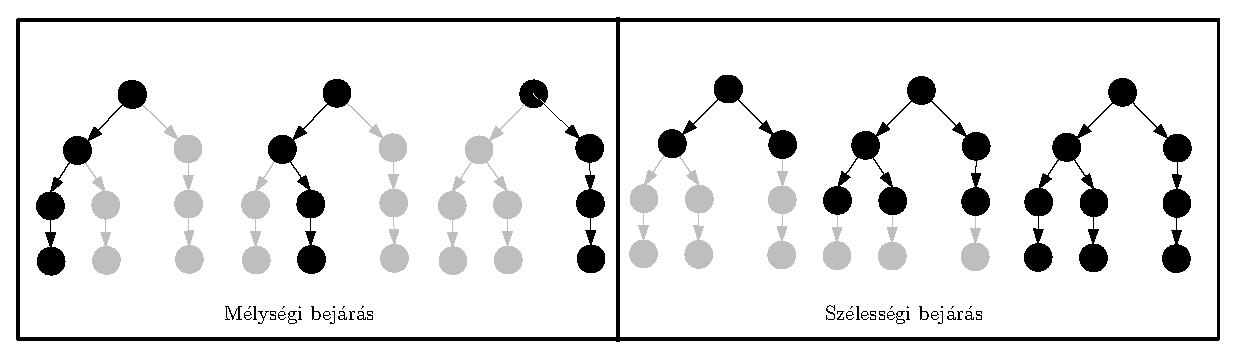
\includegraphics[width=1\textwidth]{img/memoria.eps}
	\caption{The different traverses of the Exploded Graph and the parts which 
	needs to be stored in the memory (black). Depth first search (left) and 
	breath first search (right).}
	\label{fig:bejaras_szemleltetes}
\end{figure}

Moreover, in order to use less memory during the analysis, the CSA clears the ExplodedNodes which are unnecessarily kept in the memory. This mainly means, the nodes that are created to help the analysis but not representing concrete state changes in the actual running of the program.

%%%%

